\documentclass[]{article}
\usepackage{graphicx}
\graphicspath{ {./images/} }

%opening
\title{Double-Descent}
\author{Joe Down}
\date{}

\begin{document}

\maketitle

\begin{abstract}
TODO
\end{abstract}

\section{Introduction}
The suitability of machine learning models is typically measured by evaluating some appropriate risk measure comparing predicted results with 'real' results from an unseen training dataset\cite{}. Training algorithms seek to find model parameters (and hyper-parameters) resulting in minimal risk.\\
\begin{figure}[h]
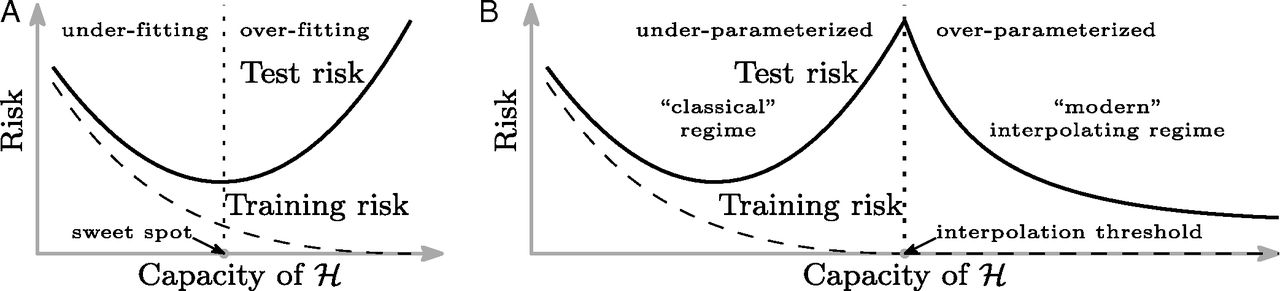
\includegraphics[width=\textwidth]{pnas.1903070116fig01}
\centering
\caption{Classical understanding of model complexity's impact on risk minimisation versus modern practical findings\cite{belkin2019reconciling}}
\label{figure:double_descent}
\end{figure}

\section{TODO}
TODO

\section{Conclusions}
TODO

\bibliography{template_Article}
\bibliographystyle{acm}

\end{document}